\section{Résolution des problèmes}

\paragraph{Résolution du problème (P) :}La reformulation de Benders précédente contient un nombre exponentiel de contraintes. Les auteurs ont donc résolu itérativement le problème maître réduit (PMR) contenant un faible nombre de contraintes (4a) associées aux points extrêmes dans $P_D$. Les contraintes sont ajoutées au fur et à mesure en résolvant les sous-problèmes duaux jusqu'à atteindre une solution optimale du problème original (P) comme indiqué dans le pseudo-code  figure \ref{alg1}.

\begin{itemize}
	\item ub désigne une borne supérieure,
	\item t : Entier caractérise les itérations successives,
	\item $P^t_D$ : Ensemble des points extrême à l'itération t, 
	\item  $MP(P^t_D)$ : Problème Maître relaxé (PMR) en remplaçant $P_D$ par $P^t_D$,
	\item $v(MP(P^t_D)$ : Valeur optimale du (PMR) à l'itération t,
	\item $z^t$ : Vecteur optimal à l'itération t,
	\item $DS(z^t)$ : Sous-problème dual (SD) pour $z^t$,
	\item $v(DS(z^t))$ : Valeur optimale du sous-problème (SD).
\end{itemize}

\begin{figure}[H]
	\begin{center}	
		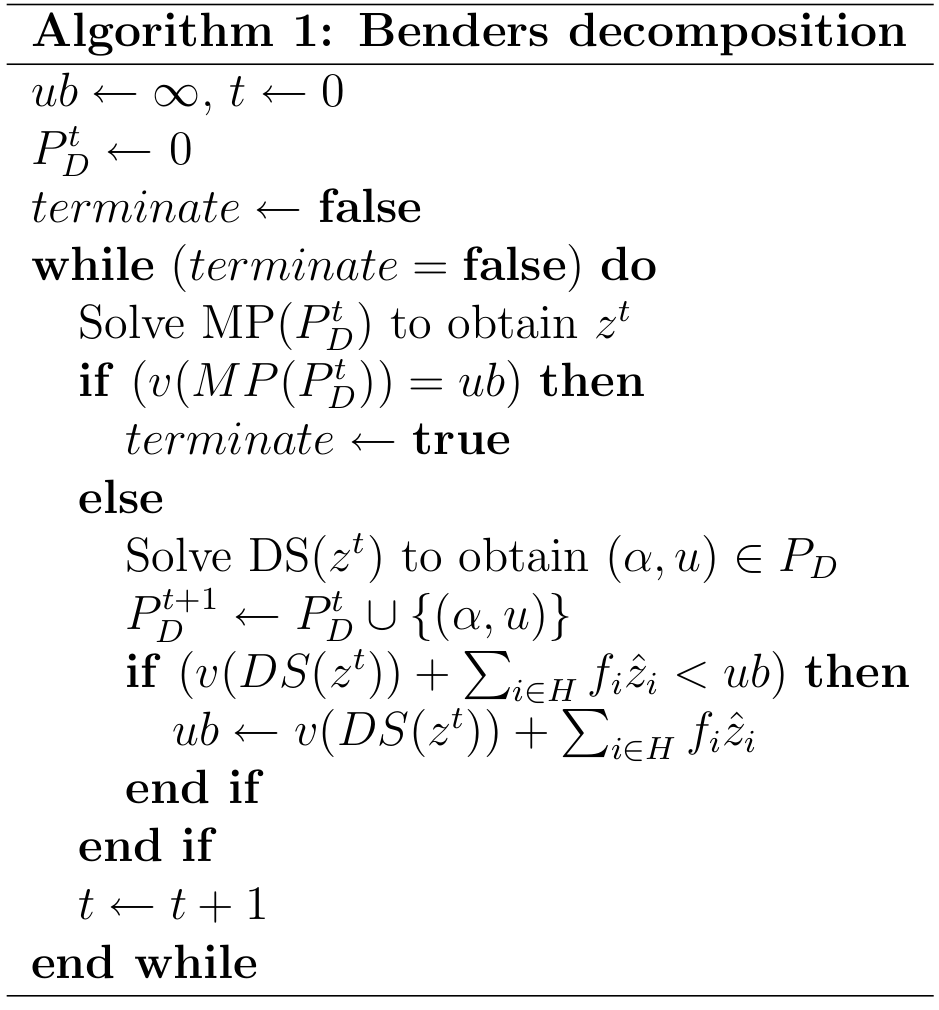
\includegraphics[scale=0.3]{images/alg1}
		\caption{Calcul de la solution optimale du problème original (P) si elle existe.}
		\label{alg1}
	\end{center}
\end{figure}


  \paragraph{Résolution de sous-problème Dual :}

L'algorithme précédent nécessite la résolution des sous-problèmes duaux $DS(z^t)$. Les auteurs utilisent une méthode qui exploite la structure du sous-problème primal en l'occurence sa \textit{décomposabilité} en card(K) sous-problèmes $PS^t_k $ plutôt qu'une résolution directe du dual à l'aide d'un solveur. Les solutions du dual $(\alpha^t, u^t)$ sont déduites du théorème complémentaire en théorie de la dualité. Ainsi à partir d'une solution optimale $x^t$ du primal $PS^t_k$, les auteurs en déduisent un ensemble noté $DO^t$ de solutions optimales du dual $DS^t$.

\paragraph{}Il s'agissait ensuite pour les auteurs de sélectionner une solution optimale $(\alpha^t, u^t)$ tirée de $DO^t$, notamment en sélectionnnant des valeurs admissibles pour les variables duales $\alpha^t_k$ et $u^t_{ek}$. Des conditions filtrantes sont aussi déterminées, en particulier, une borne inférieure des variables $u_{ik}$ notée $l_{ik}$.
Enfin, les auteurs privilégient le choix d'un vecteur dual optimal $(\alpha^t, u^t)$ qui
produira des coupes efficaces d'optimalité, en l'occurrence les vecteurs dont $u^t$ est le plus petit possible pour obtenir la plus grande borne inférieure possible pour la valeur optimale du problème maître relaxé à l'itération suivante $t+1$.

